\documentclass[12pt, a4paper]{article}
\usepackage[utf8]{inputenc}
\usepackage[default,scale=0.95]{opensans}
\usepackage[labelfont=bf]{caption}


\usepackage{fancyhdr}
\usepackage{url}
\usepackage[export]{adjustbox}

\usepackage{fancyvrb}
\usepackage{hyperref}
\usepackage{graphicx}
\usepackage{float}

\usepackage{fancybox}
\usepackage{graphicx}
\usepackage{adjustbox}
\usepackage{listings}



\hypersetup{
    colorlinks=true,
    linkcolor=blue,
    filecolor=magenta,
    urlcolor=cyan,
}


\def\myname{Sam Shahriari}
\def\assignment{Assignment 4}
\def\course{DD2424}



\author{Sam Shahriari}
\title{\course: \assignment}

\pagestyle{fancy}
\fancyhf{}
\rhead{\myname}
\chead{\assignment}
\lhead{\course}
\cfoot{ - \thepage \ -}
\renewcommand{\headrulewidth}{.1pt}


\begin{document}
\maketitle
\section{Gradient check}
To check that my gradients were correctly computed, I compared them to a numerical estimation when the network had 5 hidden nodes. This was good practice as one of the matrix multiplication calculated the inner dot product instead of the outer. After this was fixed, no difference was bigger than 1e-6. It would be appreciated if a numerical calculation of the gradients written in Python was also provided.

\begin{figure}[H]
    \centering
    \fbox{\begin{minipage}{0.5\textwidth}
            \VerbatimInput{gradient_error}
        \end{minipage}}
    \label{fig:gradient}
    \caption{Maximal errors between analytical and numerical gradients }
\end{figure}

\section{Training phase}
The training consisted of splitting the text into chunks of 25 characters and then doing stochastic gradient decent on every chunk. Gradients were updated using AdaGrad. To mitigate the high cost of calculate the loss on the whole training set, a smooth loss, a weighted average of the previous losses and the current batch loss, was used. The loss over two training epochs can be seen in \autoref{fig:loss}.

The model learns quite quickly to synthesize correct sentence structures but many of the words are just made even after 100.000 iterations, this can be seen in \autoref{fig:evolution}. When training for longer (20 epochs, smooth loss=37.2)the prediction gets much better, now most of the words are correctly spelt (\autoref{fig:20epochs}).

\begin{figure}[H]
    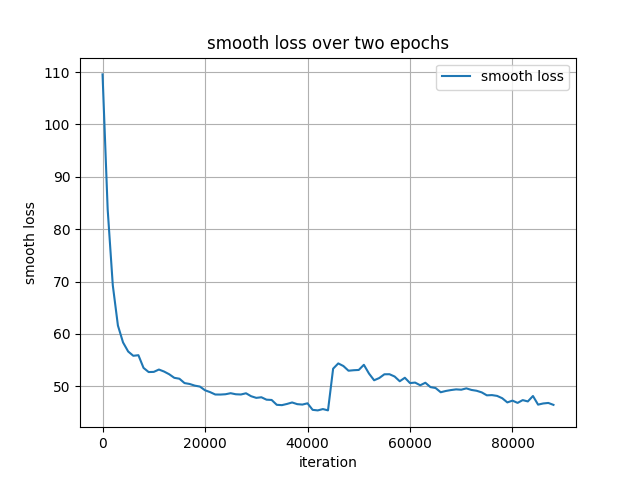
\includegraphics{smooth_loss.png}
    \caption{Loss over two epochs}
    \label{fig:loss}
\end{figure}

\begin{figure}[H]
    \centering
    \begin{adjustbox}{minipage=1.1\textwidth,fbox}
        {\scriptsize
            \lstinputlisting[breaklines]{evolution.txt}
        }
    \end{adjustbox}
    \caption{Generated text from the language model at every 10,000 iteration. }
    \label{fig:evolution}
\end{figure}

\begin{figure}[H]
    \centering
    \begin{adjustbox}{minipage=\textwidth,fbox}
        {\scriptsize

            \lstinputlisting[breaklines]{20epochs}
        }
    \end{adjustbox}
    \caption{Generated text from the language model after 20 epochs.  }
    \label{fig:20epochs}
\end{figure}



\end{document}